\chapter{Introduction}

Artificial Intelligence is defined as the study and design of intelligent systems. An intelligent system is one which perceives its environment and takes actions that maximizes its chances of success. The nature of this environment varies from system to system. For example, the environment for a chess playing system can be enumerated with a set of rules; the environment for an autonomous car is the size, position of cars, their relative speeds on the street and the position of important objects like traffic lights, stop signs. The search space of an AI problem is the total number of candidate objects over which a decision needs to made. In both the above examples, the search space contains an enormous of candidates. But for the second case, the problem of enumerating the search space is non-trivial. It requires a large amount of knowledge about the environment. Also, the interactions between elements in the real world are very hard to predict. They need to be \textit{sensed} in a real time fashion for decisions to be made accordingly. With the growing amount of sensors in the real world, its becoming possible to record events and activities of increasingly finer granularity. Sensory inputs in the real world could range from news articles on the web to stock market tickers to thermometer readings from wildlife parks. Such a large amount of heterogeneous information cannot be easily stored, processed and analyzed. 

This dissertation addresses the problem of constructing computational representations of real world environments from various heterogeneous sensors, to reason which parts of the search space can be pruned without hurting the overall performance of the intelligent system. We refer to such a representation as the \textbf{Context Network} of the environment. The network describes real-world events occurring in the environment, the entities participating in them, and their semantic inter-relationships.

\begin{figure}[t]
\centering
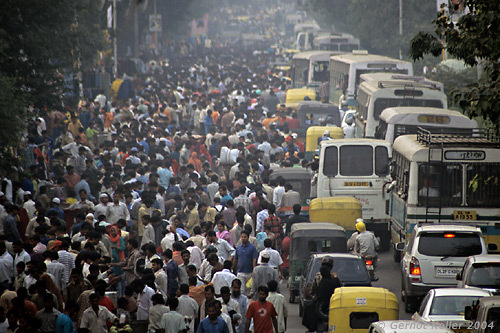
\includegraphics[width=0.75\textwidth]{media/chapter1/india-streets.jpg}
\caption{Such streets would pose a significant challenge in designing automomous cars.}
\label{fig:india-streets}
\end{figure}

\section{Approach}
Before embarking on a mission to model the entire world, we ask ourselves the question: How much of the real world information is actually relevant to the intelligent system? Constructing the entire world model is extremely challenging and often unnecessary. For example, there might not be much value in representing sports events in New York in a model being used to help cars navigate in Japan. 

\begin{figure}[t]
\centering
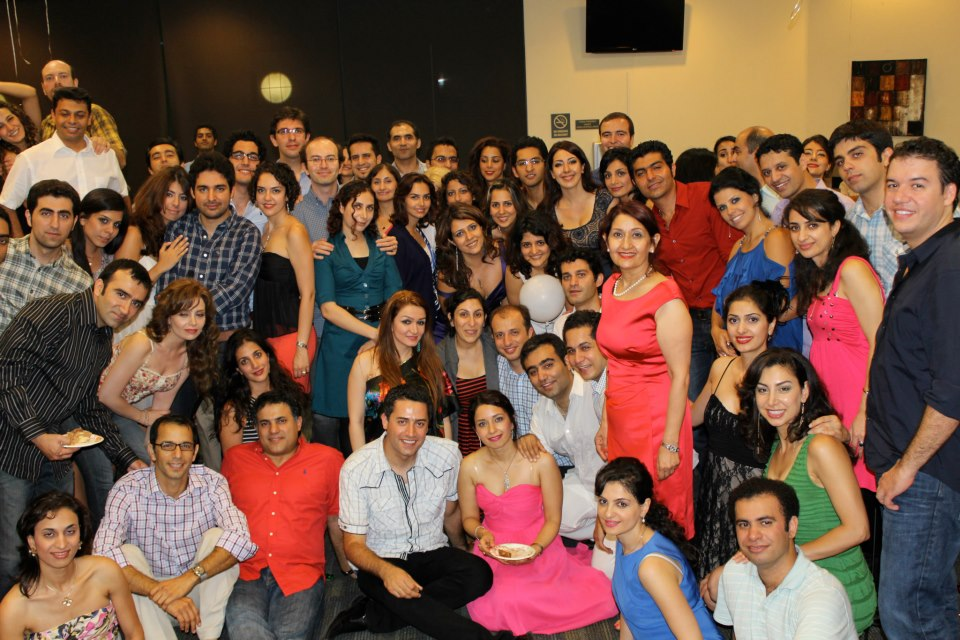
\includegraphics[width=\textwidth]{media/chapter1/setarehetal.png}
\caption{Face tagging problems could be challenged by very large search spaces.}
\label{fig:india-streets}
\end{figure}

This primary \uline{contribution} of this dissertation is a \textbf{\textit{progressive discovery}} algorithm to ingest information from various real world data sources to construct context networks containing the most relevant information for pruning the search space for the system. Examples of data sources include social media web services to provide information about events and entities like Facebook, Twitter; services which can be queried to find information about places like Yelp; Sensors on personal mobile phones, for example GPS which inform applications of the location of a person is present at any given point in time.

\textbf{What is progressive discovery?} Progressive discovery is an incremental process where knowledge of real world events and entities can be added to a given context network. If we look at this definition recursively, it says that given a context network and some data sources describing events and entities, a progressive discovery algorithm will obtain new information from the sources and relate it to context network. By repeatedly executing this algorithm, we can grow a context network until the data sources can provide no further information or the information in the network prunes the search space well enough for the AI problem to be fully solved.

In the following chapters, discussion on context networks, and their discovery from various data sources will be presented in conjunction with an application to \textbf{tag faces in personal photos}. The face tagging algorithm, whose search space contains a few billion entities is a very hard real world AI problem. But if a real world model of the world existed, the search space which is relevant to this photo contains just the entities who are present within the field of view of the camera at the time the photo was captured. 

\section{Why Prune Search Spaces?}
Search space pruning has been identified as an important problem since the earliest discussions on Computer Science topic. So what has changed in the last few years, that we should focus on it again? The following reasons describe, in a nutshell, the differences between this problem and previously tackled problems and why it is relevant today.

First, the application of computer science is no longer restricted to abstract algorithms but the real world. Systems working on the problems like autonomous car navigation and personal photo tagging. Sensors are deployed around the world to tap into real world information. The challenges in integrating many, different types of sensors provides a new research opportunity.

Second, systems are working against a very large audience. It is quite clear with the emergence of personalization techniques that it is not possible to use the same hammer against all users' problems. These people come from various cultures, different backgrounds and unique needs. Knowledge of real world information most relevant to each user is becoming increasingly desirable to solve their individual problems. This desiderata requires looking at the search space pruning in a different light.

Third, original pruning solutions worked against very hard problems like Chess playing agents, where the very large search space was enumerated through a rule based system. It can be argued that due to the simplistic model, it was harder to prune the space as there were no properties which could be exploited to do so. But by bringing in real world, we can bring in more variables into the picture, and therefore more \textit{relations} can be exploited to prune the search space.

In summary, it can be said that large availablilty of personal, social and sensor information, and the need to incorporate real world semantics, change the dynamics of search space pruning problems, and it must be visited so new solutions can be designed for current problems.

\section{Overview}
This dissertation is organized into the following chapters. Chapter 2 provides an overview of context, how context has been used to address problems in various scientific disciplines and how we use context in our specific personal photo tagging application. Chapter 3 describes the related work in computer science, and how this work is informed by them. Chapter 4 describes our context discovery framework, how it models various data sources, and how our progressive discovery algorithm constructs models for real world problems. We facilitate this discussion with an example real world application to tag faces of people in personal photos. Chapter 5 analyzes the algorithmic complexity of different parts of the system, and provides experiments to verify the competence and performance of the system. We also present experiments to confirm the efficacy of our approach in the light of the real world application. Finally, chapter 6 attempts to describe the future possibilities of using context discovery in computer science.

% Chapters 6 and 7 describe two extensions to the CueNet framework to solve problems of missing context and that of source selection. 

\section{Terminology}
Before starting the discussion on Context Networks, it is necessary to include this short note on terminology to avoid any ambiguities. We use the word `Object' to collectively refer to events and entities. An entity includes persons, places in the world, for example `Starbucks, UC Irvine', `The Eiffel Tower, Paris, France', or organizations, for example `Google Inc', `Royal Society of London'. `Object' has been used in literature to refer to things which have no spatio-temporal properties. But, in our discussion, an `object' could imply an event which exhibits spatio-temporal properties.

